\documentclass[12pt,a4paper]{article}
\usepackage[utf8]{inputenc}
\usepackage{graphicx}
\usepackage{geometry}
\geometry{left=3cm,right=2.5cm,top=2.5cm,bottom=2.5cm}
\usepackage{setspace}
\usepackage{hyperref}
\usepackage{booktabs}
\usepackage{float}
\usepackage{caption}
\usepackage{amsmath}
\usepackage{enumitem}
\usepackage{longtable}
\usepackage{booktabs} 
\usepackage{array}
\usepackage{xcolor}
\usepackage{colortbl}
\newcommand{\rupee}{\textrupee}
\definecolor{lightgray}{gray}{0.93}

\setlength{\parskip}{0.8ex}
\renewcommand{\baselinestretch}{1.1}

\begin{document}

%--------------------------------------
% Title Page
%--------------------------------------
\begin{titlepage}
\centering

\includegraphics[width=5cm]{iitb.eps}\\[0.8cm]

{\bfseries\Large Indian Institute of Technology Bombay}\\[1.2cm]
{\Large \textbf{Application for Ethical Clearance}}\\[1.2cm]

{\bfseries\LARGE JoDo: Joy of Digital cOntrol\par}
\vspace{0.4cm}
{\Large Evaluating a Launcher-Integrated Reward System for Mindful Smartphone Use and Digital Wellbeing\par}

\vspace{1.8cm}
\begin{tabular}{rl}
\textbf{Principal Investigator:} & Hariom Mewada (Roll No. 24M2137)\\
\textbf{Faculty Advisor:} & Prof. Bhaskaran Raman\\
\end{tabular}

\vfill
{\large October 2025}

\end{titlepage}

\newpage
\tableofcontents
\newpage

\section{Background and Rationale}
Excessive and unregulated smartphone use is an increasing documented concern in academic and public health literature.Existing digital well-being interventions predominately rely on restriction-based mechanism such as timer,app-blocking, and lockout.Research has consistently shown that such approaches undermine user autonomy,trigger psychological reactance,and fail to produce lasting behavior\cite{ko2015, Roffarello2023}.

This study evaluates \textbf{JoDo (Joy Of Digital cOntrol)}, a novel Android launcher application developed at IIT Bombay that takes fundamentally difference approach:rather than restricting access,JoDo promotes mindful smartphone usage through a launcher-integrated reward system,real time usage transparency,friction at the point of app access,and social competition via leader-boards.The system is grounded in principal of digital minimalism,intrinsic and extrinsic motivation theory,and prior HCI research on entry point intervention.
The central research question driving this study is: \textit{How can a launcher integrated reward system promote mindful smartphone usage while preserving user autonomy?}

\section{Study Objectives}
The specific objective of the study are to:
\begin{enumerate}
    \item Evaluate the effect of \textbf{JoDo} on participants' daily smartphone usage pattern for a two-week period.
    \item Assess changes in participants' psychological well-being, specifically positive and negative affect,before and after using JoDo.
    \item Examine how competition and leaderboard rank interact with participants' daily sense of motivation,stress,and self-control.
    \item Understand participants' subjective experience of autonomy,fairness,and engagement with reward system.
    \item Identify design implications for future digital well-being tools that integrate motivation and social dynamics.
\end{enumerate}
\section{Study Design}
This is a \textbf{single arm,observational deployment study} with no control condition.It is not a clinical trial and does not involve any medical intervention,deception,or withholding of treatment.The study follows a three phase design: 
\begin{enumerate}
    \item \textbf{Phase 1 - Entry (Day 0):}participants complete a validated on-boarding survey (approximately 20 minute) covering demographic information,prior digital well-being tool experience,self-control traits(BSCS),self-regulation tendency(SSRQ),and baseline semotional well-being (PANAS-SF).Following the survey,participants' attend a 30-45 minute semi-structured vedio interview and are onboarded onto JoDo.
    \item \textbf{Phase 2 - Deployment (Day 1 - 14):}Participants use JoDo as their default Android launcher for 14 consecutive days.JoDo automatically logs screen time, unlock count, and app launch count.Each evening participants complete a short daily survey(5-7 minutes) covering satisfaction,self-control,stress,focus,leaderboard rank perception, and open-ended reflection. An optional mid-point check-in is offered on Day 7.
    \item \textbf{Phase 3 - Exit (Day 15):}Participants compelte an exit survey repeating the PANAS-SF, BSCS, and SSRQ instruments, and additioally complete the System Usability Scale(SUS) and Intervention Appropriateness Measure(IAM).They then attend a 30-45 minute semi-structured exit interview.
\end{enumerate}
\section{Participants Recruitment}
\textbf{Target sample size:}20-25 participants(following prior comparable studies in this space, e.g. \cite{karthik2026}, N = 25)

\textbf{Eligibility criteria:}
\begin{itemize}
    \item 18 years of age or older
    \item Currently enrolled college student(UG,PG, or PhD)
    \item Uses and Android smartphone as a primary device
    \item Able to commit for 14 days of participation
    \item Available for 2 vidio call interviews
\end{itemize}
\textbf{Exclusion criteria:}
\begin{enumerate}
    \item iOS user(JoDo is Android-only)
    \item Individuals currently participating in another digital well-being study
    \item Individuals who report a current diagnosis of a mental health condition that may be exacerbated by reflection on technology use(self-reported on interest form)
\end{enumerate}

\subsection{Pilot study user feedbacks}
\begin{enumerate}
    \item Change the default timer value if user click I am bored change it 30 minutes, and user click if am working change to 10 minutes.
\end{enumerate}
\subsection{New Questions}
\begin{enumerate}
    \item Why Being HomeScreen(Fully minimalist and less visual cues) disliked by users?
\end{enumerate}
\section{Feb 26 (last meeting) - Mar 04 2026}
{ \bf No. of Hours: 20}
\subsection{List of Task Completed}
\begin{enumerate}
    \item Created a python Script to retrieve pilot study data from db and generate graphs and insights over them.
    \item Fixed bugs and verified script output.
    \item Generated pilot Study data analysis report (\href{https://drive.google.com/file/d/1GWn26HUfRNxbJ2xH5aLeTd6d8hEtVdlX/view?usp=sharing}{link}).
    \item Collected log file from pilots phone.
    \item In one device found Home screen was crashing due to Integer overflow exception.
    \item App was crashing on Device BootUp in pilots phone.
    \item Prepared new UI design proposal for HomeScreen, Lock Screen and App Drawer.
    \item Created Google form  (\href{https://forms.gle/D1U46AeNB6NzSw1fA}{link}) for post pilot study feedback, similar to what Omkar used for Intentor user study.
    \item Collected response from all the participants.
\end{enumerate}
\subsection{Proposed new UI for JoDo}
\subsubsection{Problem in the current UI}
\begin{enumerate}
    \item It looks like old school.
    \item Progress bar has occupied to much space and it is the main cause of so runtime exceptions in the HomeScreen.
    \item Current UI not properly reflect out Psychology of \textbf{JoDo} as well as \textbf{Digital Minimalism}
\end{enumerate}
\subsubsection{Proposed UI Prototypes:}

\begin{figure}[H]
    \centering
    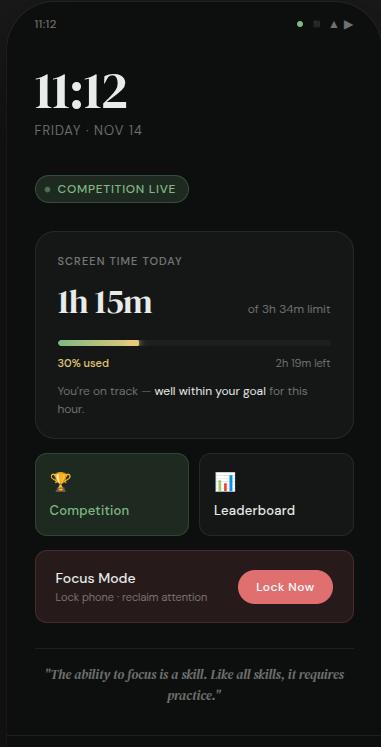
\includegraphics[width=0.45\linewidth,height=0.50\textheight, keepaspectratio]{JoDo new UI design/HomeScreen.png}
    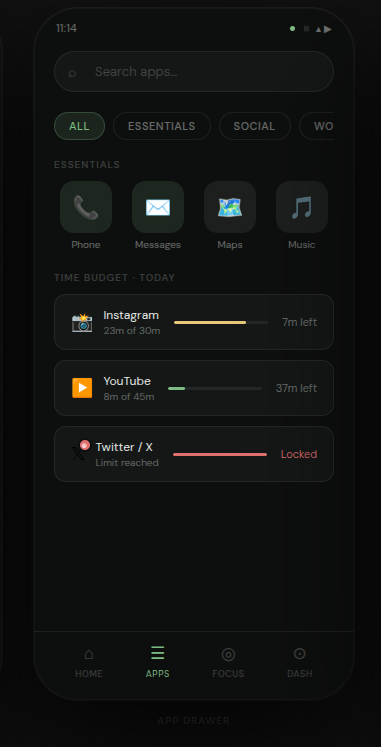
\includegraphics[width=0.45\linewidth, height=0.50\textheight, keepaspectratio]{JoDo new UI design/App_drawer.png}

  %   \vspace{0.3cm}

    % 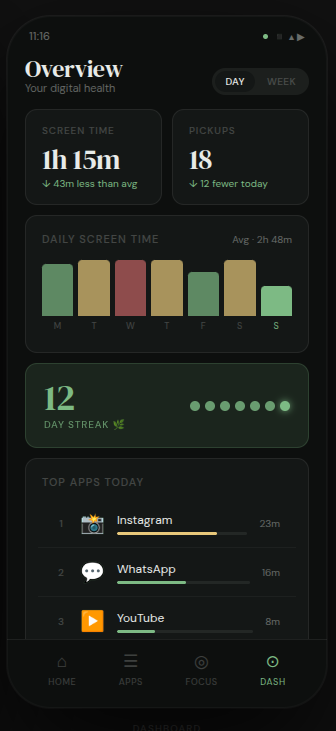
\includegraphics[width=0.45\linewidth]{JoDo new UI design/dashboard.png}
    % 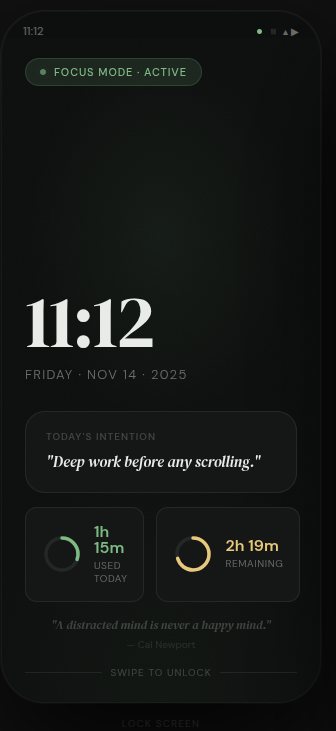
\includegraphics[width=0.45\linewidth]{JoDo new UI design/lock_screen.png}

    \caption{Home-screen(left), App-drawer(right)}
    \label{fig:ui_prototype}
\end{figure}


\begin{figure}[H]
    \centering
    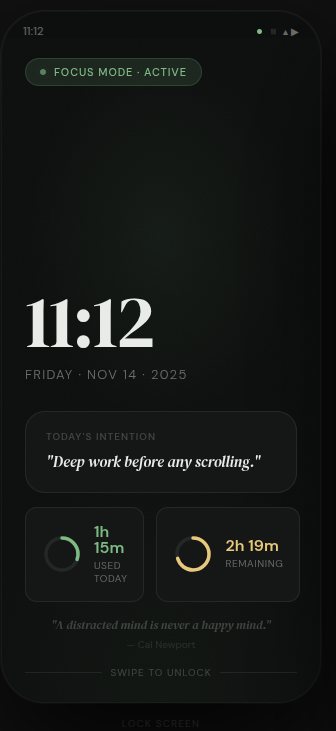
\includegraphics[width=0.45\linewidth,height=0.50\textheight, keepaspectratio]{JoDo new UI design/lock_screen.png}
    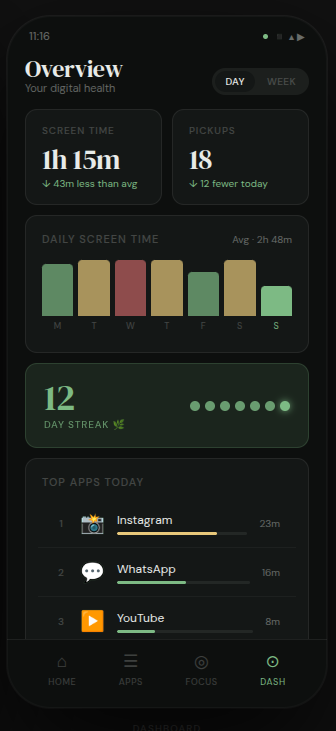
\includegraphics[width=0.45\linewidth, height=0.50\textheight, keepaspectratio]{JoDo new UI design/dashboard.png}

   % \vspace{0.3cm}

    % 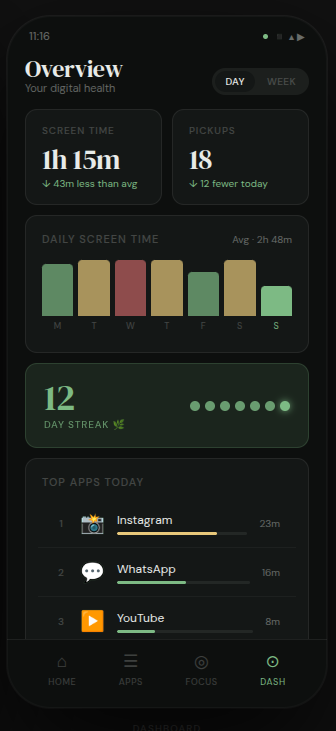
\includegraphics[width=0.45\linewidth]{JoDo new UI design/dashboard.png}
    % 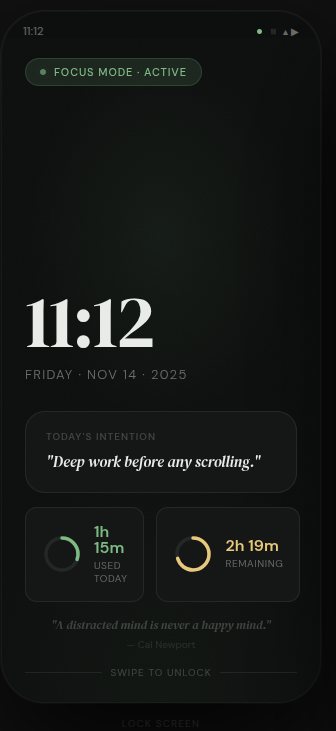
\includegraphics[width=0.45\linewidth]{JoDo new UI design/lock_screen.png}

    \caption{Lock-screen (left), DashBoard (right)}
    \label{fig:ui_prototype}
\end{figure}

\subsection{To Do}
\begin{enumerate}
    \item Create summary for qualitative analysis through the response recieved in google form from all the 3 participants.
\end{enumerate}
\subsubsection{JoDo economy similar to \href{https://play.google.com/store/apps/details?id=in.sweatco.app&pcampaignid=web_share}{Sweat Coin App}}
\begin{enumerate}
    \item Create JoDo Economy similar to sweatcoin, they convert steps into real money (but their rewards are virtual ). 


\begin{figure}[H]
\centering
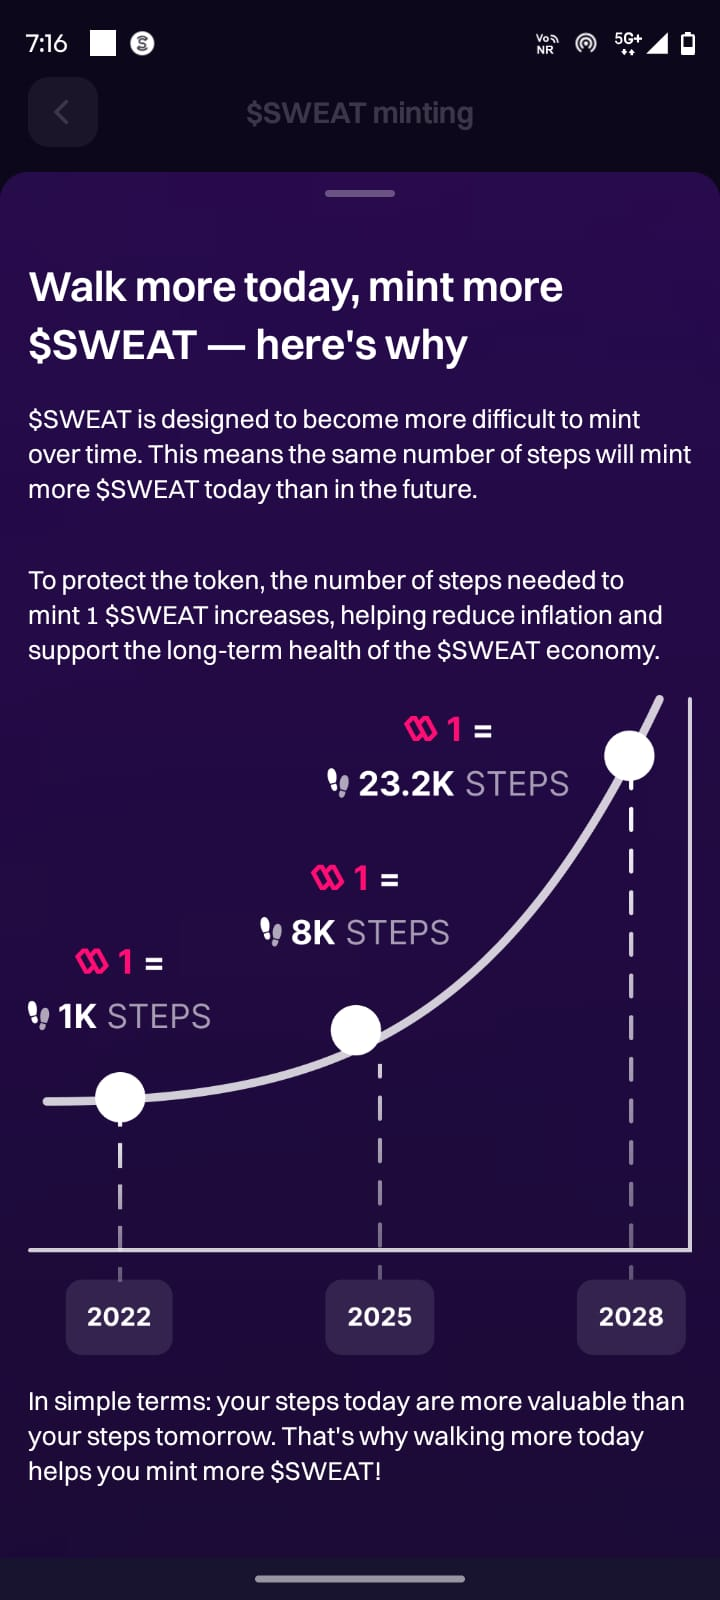
\includegraphics[width=0.45\linewidth,height=0.50\textheight, keepaspectratio]{sweat_coin_app_UI.jpeg}
   \caption{UI interface from Sweat Coin app}
    \label{fig:sweat_coin_app_UI}
\end{figure}
\end{enumerate}
\section{Mar 02 2026 - Mar 09 2026}
{\bf No. of Hours: 20}

\subsection{UI Changes}
\begin{enumerate}
    \item Create new UI for Homescreen, Appdrawer and LockScreen.
    \item Made all the buttons function in the new UI.
    \item Reflected real usage from device.
    \item Resued all the existing fuctionality from the app and only changed the UI.
\end{enumerate}
\begin{figure}[H]
    \centering
    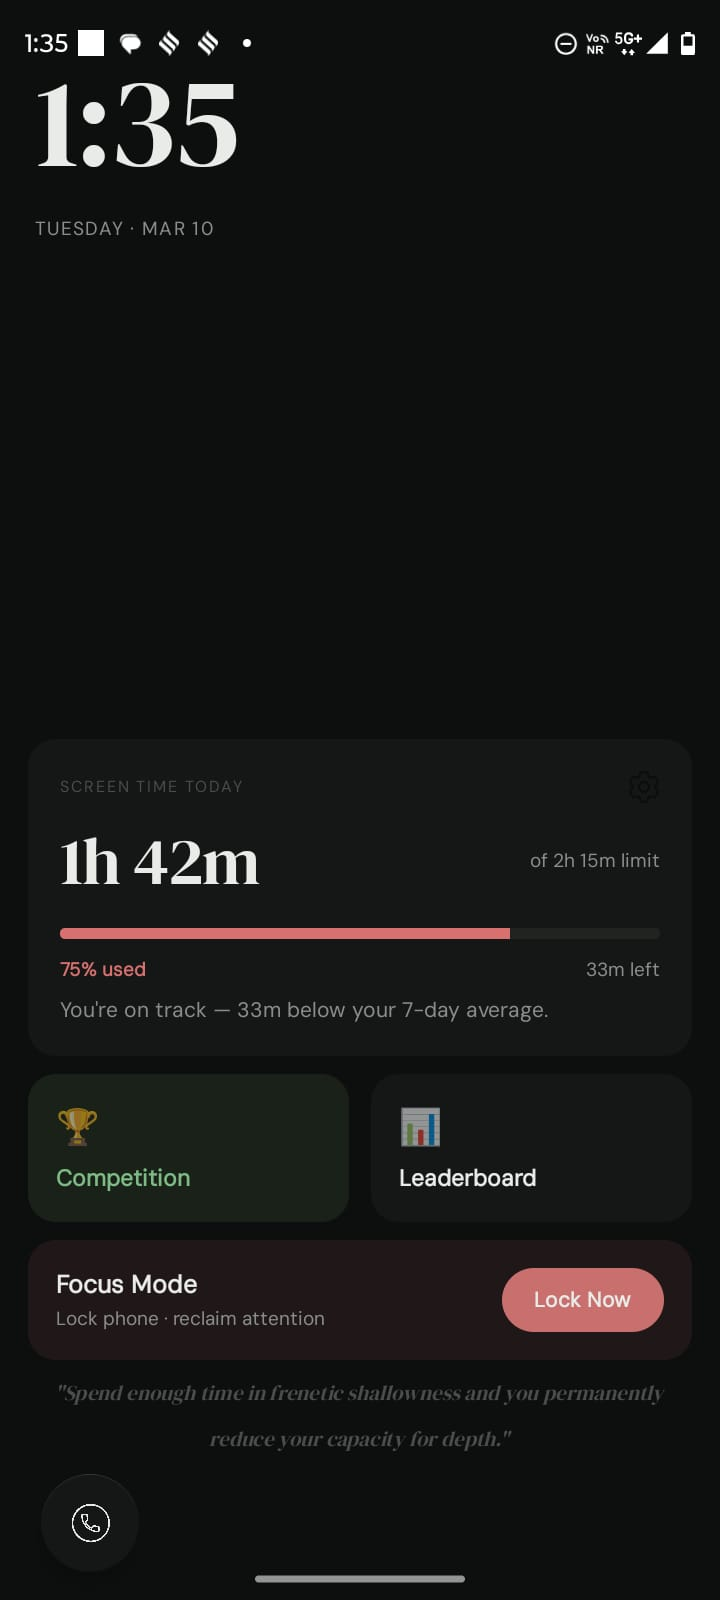
\includegraphics[width=0.50\linewidth,height=0.50\textheight, keepaspectratio]{home_screen_new.jpeg}
    \hspace{0.3cm}
    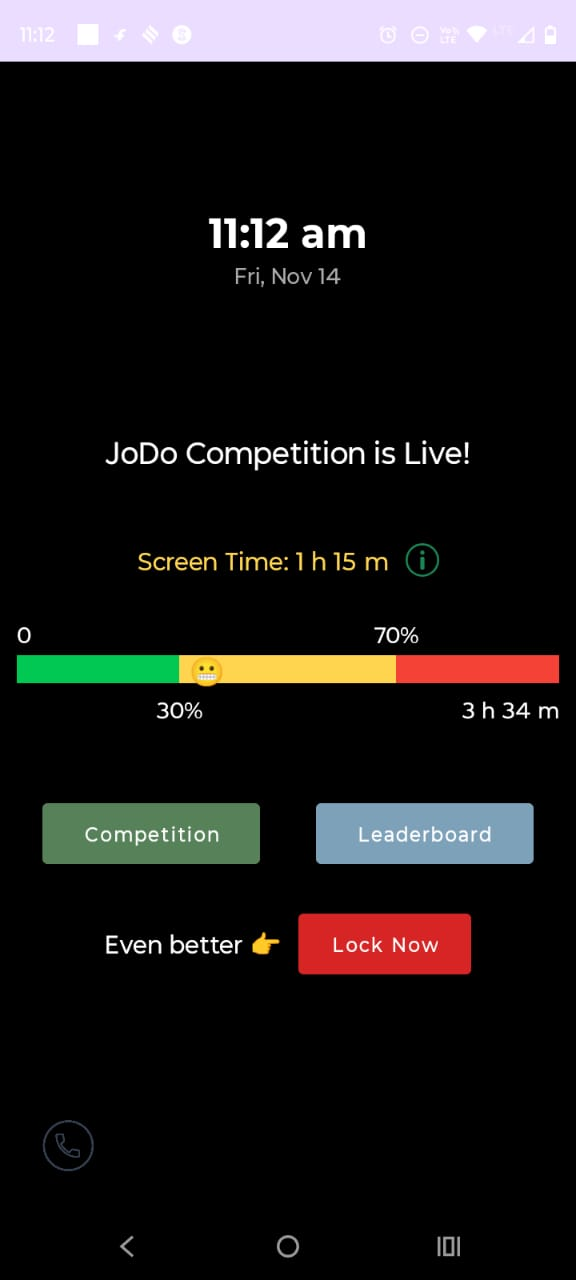
\includegraphics[width=0.50\linewidth, height=0.50\textheight, keepaspectratio]{home-screen-old.jpeg}

    % \vspace{0.5cm}

    % 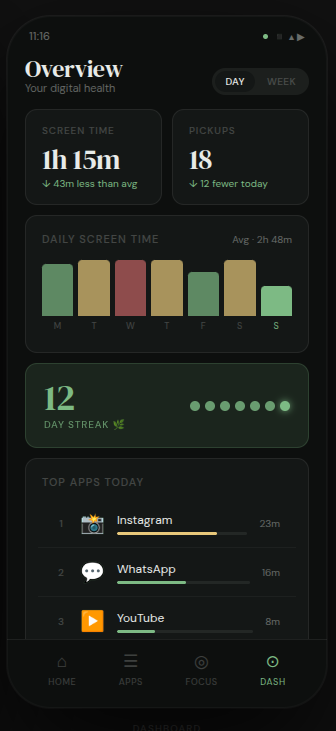
\includegraphics[width=0.45\linewidth]{JoDo new UI design/dashboard.png}
    % 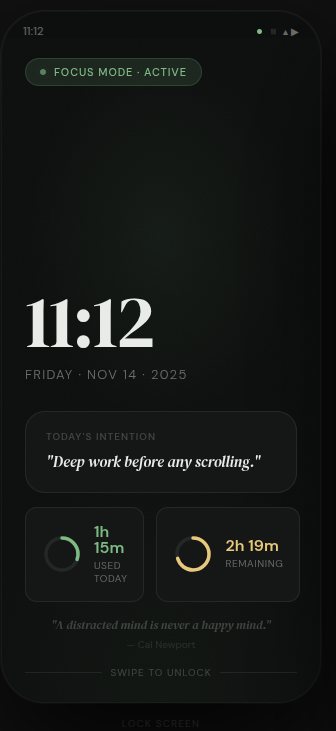
\includegraphics[width=0.45\linewidth]{JoDo new UI design/lock_screen.png}

    \caption{Home-screen-new(left),Home-Screen-old(right)}
    \label{fig:ui_prototype}
\end{figure}

\begin{figure}[H]
    \centering
    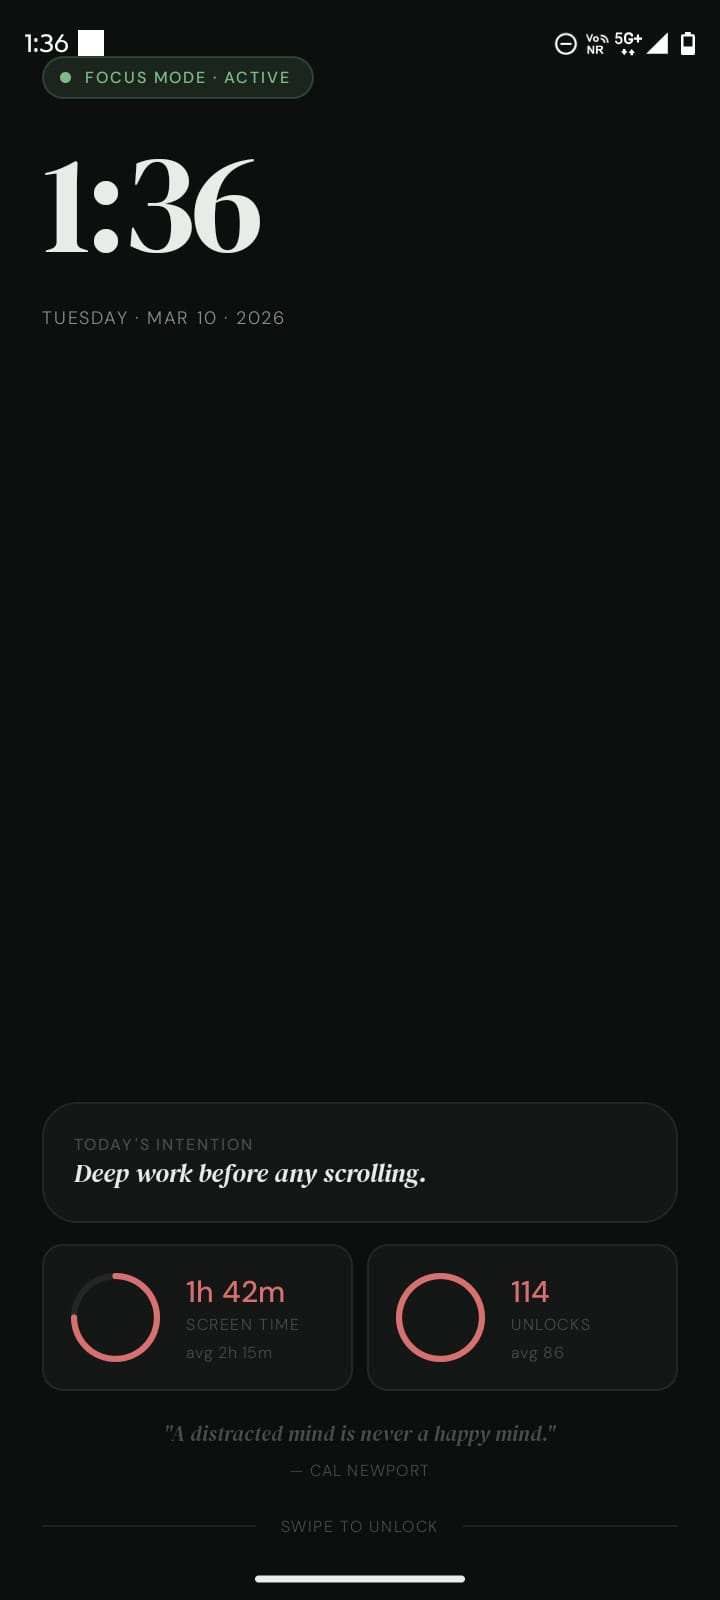
\includegraphics[width=0.50\linewidth,height=0.50\textheight, keepaspectratio]{lock_screen_new.jpeg}
    \hspace{0.3cm}
    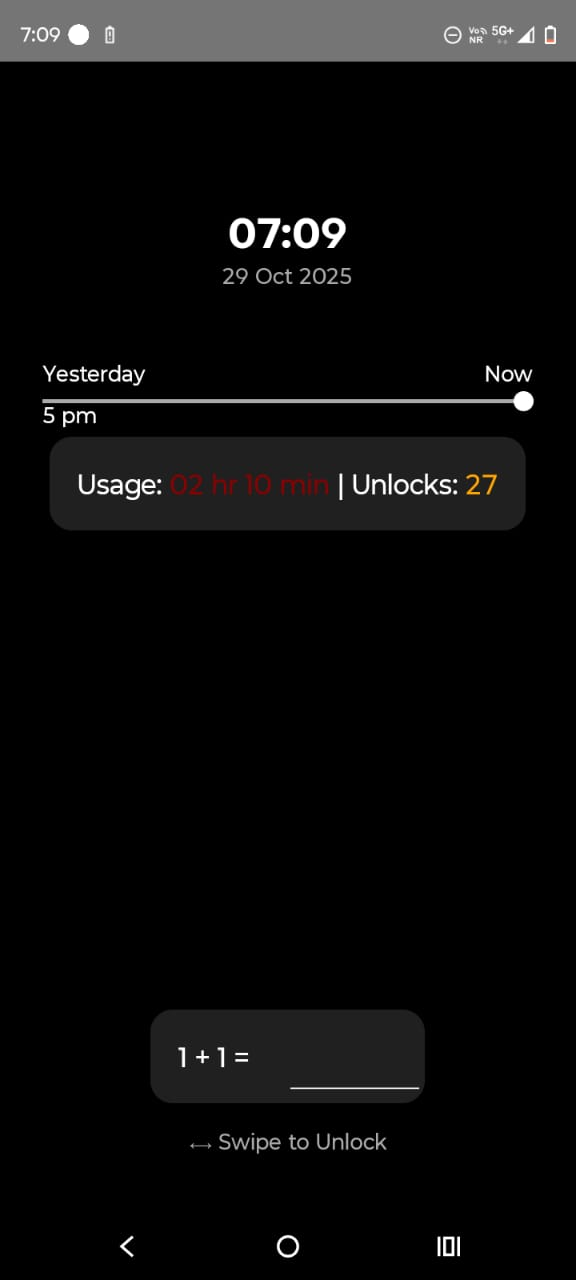
\includegraphics[width=0.50\linewidth, height=0.50\textheight, keepaspectratio]{lock-screen-old.jpeg}

    % \vspace{0.5cm}

    % 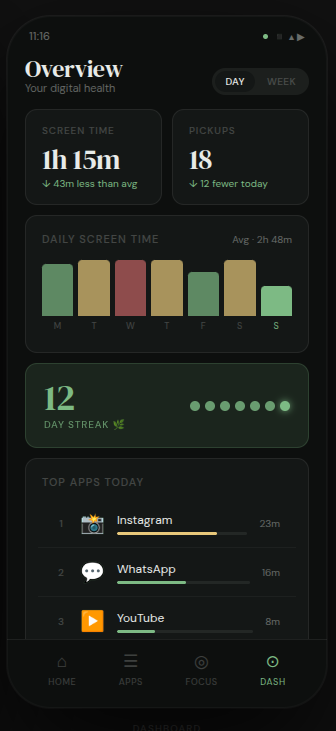
\includegraphics[width=0.45\linewidth]{JoDo new UI design/dashboard.png}
    % 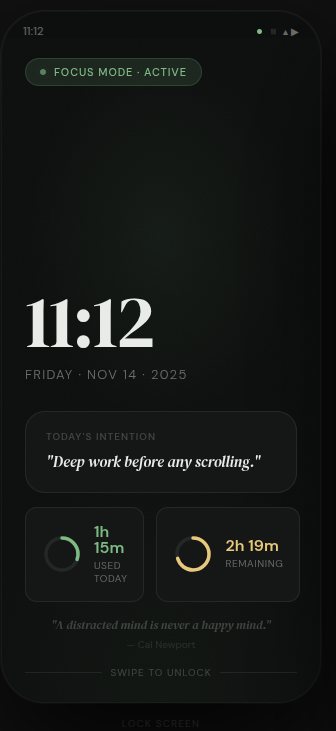
\includegraphics[width=0.45\linewidth]{JoDo new UI design/lock_screen.png}

    \caption{Lock-screen-new(left),Lock-Screen-old(right)}
    \label{fig:ui_prototype}
\end{figure}


\begin{figure}[H]
    \centering
    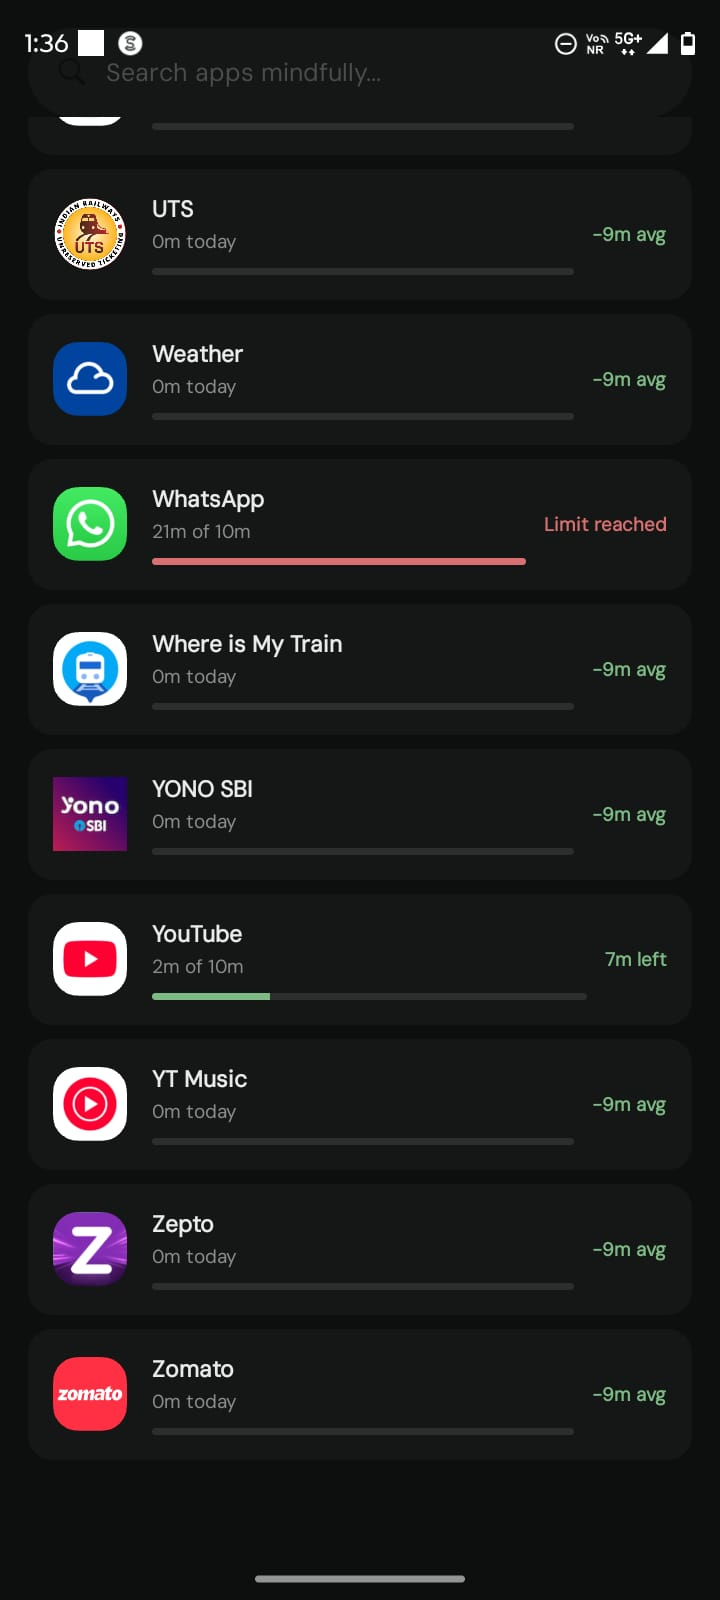
\includegraphics[width=0.50\linewidth,height=0.50\textheight, keepaspectratio]{App_drawer_new.jpeg}
%    \hspace{0.3cm}
    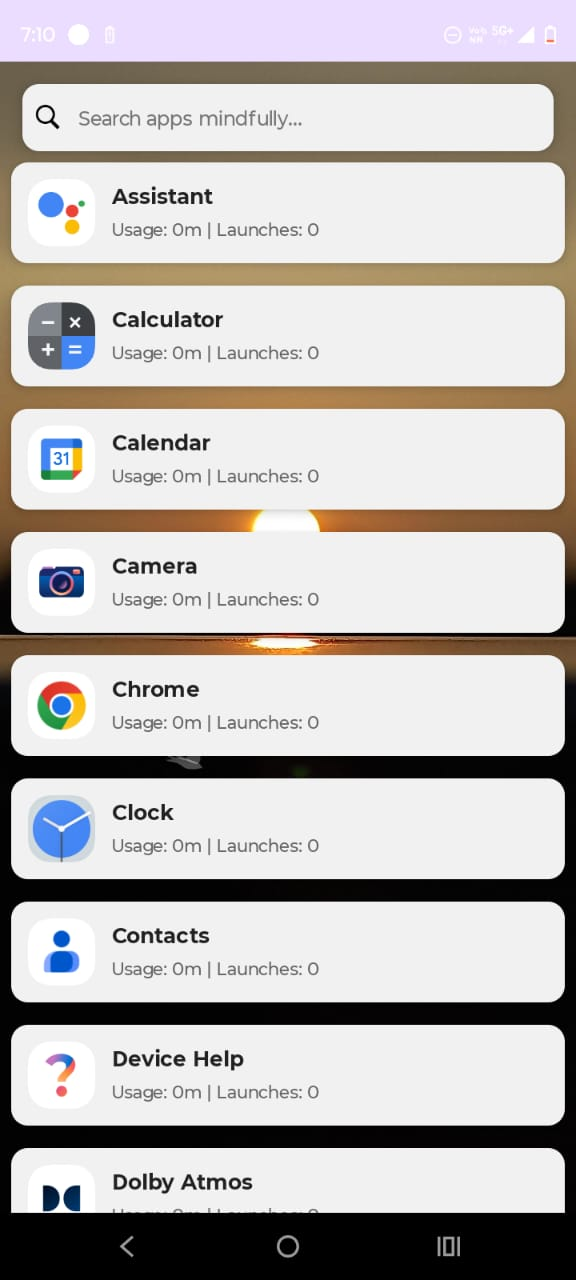
\includegraphics[width=0.50\linewidth, height=0.50\textheight, keepaspectratio]{app-drawer-old.jpeg}

   %  \vspace{0.5cm}

    % 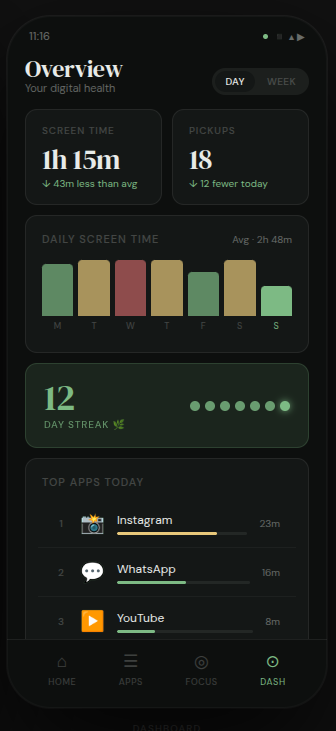
\includegraphics[width=0.45\linewidth]{JoDo new UI design/dashboard.png}
    % 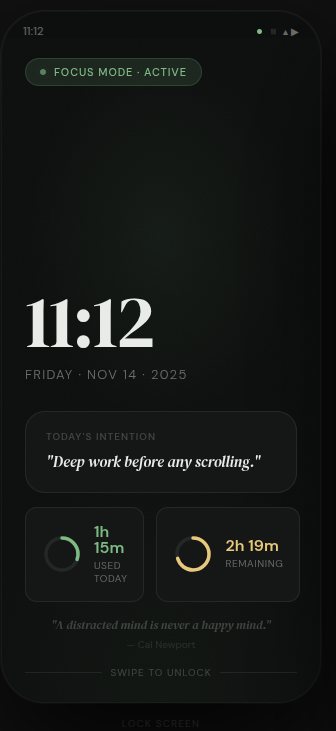
\includegraphics[width=0.45\linewidth]{JoDo new UI design/lock_screen.png}

    \caption{AppDrawer-screen-new(left),AppDrawer-Screen-old(right)}
    \label{fig:ui_prototype}
\end{figure}

\clearpage
\subsection{Pilot Study: Post-Intervention Survey Results}

A follow-up survey was administered to three participants after the pilot study using a mixed-methods instrument combining SUS-inspired Likert items and open-ended qualitative questions.

\subsubsection{Quantitative Summary}

\begin{table}[H]
\centering
\caption{Likert Response Summary (1 = Strongly Disagree / Never, 5 = Strongly Agree / Always)}
\renewcommand{\arraystretch}{1.3}
\begin{tabularx}{\textwidth}{|X|c|c|c|}
\hline
\textbf{Statement} & \textbf{P1} & \textbf{P2} & \textbf{P3} \\
\hline
JoDo is helpful in taking control over digital habits & 5 & 4 & 4 \\
\hline
I found the system unnecessarily complex & 1 & 2 & 4 \\
\hline
I thought the system was easy to use & 3 & 4 & 2 \\
\hline
I would need technical support to use this system & 1 & 2 & 2 \\
\hline
The functions were well integrated & 5 & 3 & 4 \\
\hline
There was too much inconsistency in the system & 1 & 3 & 1 \\
\hline
\textbf{Likelihood to recommend (out of 10)} & \textbf{10} & \textbf{8} & \textbf{7} \\
\hline
\end{tabularx}
\end{table}

\noindent All three participants rated JoDo positively for helpfulness (mean = 4.3/5) and expressed willingness to recommend it (mean = 8.3/10). Perceived complexity varied: P1 found the system simple and well-integrated, while P3 found navigation more demanding, particularly when the launcher was active and direct app access was restricted by design.

\subsubsection{Qualitative Themes}

\noindent\textbf{Awareness and behaviour change.} All three participants reported increased awareness of their phone usage. P2 noted that the pre-launch warning reduced impulsive social media access. P3 observed a reduction in YouTube usage, attributing it partly to the friction introduced by the launcher's search-first navigation and partly to leaderboard motivation.

\noindent\textbf{Gamification as motivator.} The leaderboard and points system were the most frequently praised features across all three responses. P3 explicitly cited the desire to rank first as a driver of sustained engagement with the challenge.

\noindent\textbf{UI and design feedback.} Two participants flagged the interface as visually dated and inconsistent with the dark theme. P2 described the design as ``old-school'' and noted that dashboard icons did not match the black colour scheme — directly motivating the UI redesign documented in the previous section.

\noindent\textbf{Bugs and accuracy.} P2 identified two technical issues: unlock count inflation due to power-button presses being registered as unlocks, and the ability to bypass app restrictions through alternative routes. Both are noted as items for the next development iteration.

\subsubsection{Summary}

The pilot study confirmed that the core JoDo mechanisms - usage warnings, the launcher-as-friction model, and competitive leaderboards — produce measurable awareness and self-reported behaviour change even in a small three-participant cohort. The primary actionable feedback was the need for a modern, consistent UI (addressed in \$3) and improved unlock-detection accuracy.

\section{Mar 09 2026 (last meeting) - Mar 13 2026}
{\bf No. of Hours: 12}
\subsection{Offline Reward}
\begin{enumerate}
    \item Created JoDo passport similar to the passport that people visit countries and get stamp of that country, we can also follow similar kind of approach whenenver people visit a place and do offline activity in IIT they get stamped and have memory offline memories. \href{https://drive.google.com/file/d/1oMPdChhu_n5pfZ2k6dNrNa-poAVlBPzW/view?usp=sharing}{link}
\end{enumerate}
\subsection{To Do}
\begin{enumerate}
    \item Implement Security measures to prevent \textbf{Denial of Service} and \textbf{Brute Force} attack.
    \item Implement Throttling and rate limit at API level as well as global throttle limit. Throattles indicate a temporary state, and are used to control the rate of request that client can send.
    \item Use \textbf{Nginx + django-ratelimit + Redis} - that covers 90\% of real-world DoS scenarios without needing paid services.
\end{enumerate}
\subsection{Steps to achieve Rate limit in Django Server}
\begin{enumerate}
    \item Set up application level rate limit using \textbf{django-ratelimit} Libraty.
    \item Setup nginx proxy, easy and very powerful can handle large number of connection concurrenly and drop the over rate limit request before they reach the django server.
    \item Use radis cache as backend server to store the Throttling class provided by Django-ratelimit.
\end{enumerate}
\subsection{Completed Work}
\subsubsection{Throttling Implementation from Django Rest Framework (Inbuilt - Library)}
\begin{enumerate}

    \item Throttling is similar to \textbf{Permission}, in that it determines if a request should be authorized or not.
    \item As with permissions, multiple throttles may be used. Our API might have a restrictive throttle for unauthenticated requests, and a less restrictive throttle for authenticated requests.
    \item The application-level throttling that REST framework provides should not be considered a security measure or protection against brute forcing or denial-of-service attacks. Deliberately malicious actors will always be able to spoof IP origins. In addition to this, the built-in throttling implementations are implemented using Django's cache framework, and use non-atomic operations to determine the request rate, which may sometimes result in some fuzziness.
    \item The application-level throttling provided by REST framework is intended for implementing policies such as different business tiers and basic protections against service over-use.
\end{enumerate}
\subsubsection{How throttling is determined}
\begin{enumerate}
    \item As with permissions and authentication, throttling in REST framework is always defined as a list of classes.
    \item Before running the main body of the view each throttle in the list is checked. If any throttle check fails an exceptions.Throttled exception will be raised, and the main body of the view will not run.
\end{enumerate}
\subsubsection{How clients are identified}
\begin{enumerate}
    \item The \textbf{X\-Forwarded-For} HTTP header and \textbf{REMOTE\_ADDR\ WSGI} variable are used to uniquely identify client IP addresses for throttling. If the X-Forwarded-For header is present then it will be used, otherwise the value of the \textbf{REMOTE\_ADDR} variable from the WSGI environment will be used.
    \item If we need to strictly identify \textbf{unique client IP addresses}, we'll need to first configure the number of application proxies that the API runs behind by setting the \textbf{NUM\_PROXIES} setting. This setting should be an integer of zero or more. If set to \textbf{non\-zero} then the client IP will be identified as being the last IP address in the X\-Forwarded-For header, once any application proxy IP addresses have first been excluded. If set to zero, then the \textbf{REMOTE\_ADDR} value will always be used as the identifying IP address.
\end{enumerate}
\subsubsection{Setting up the cache}
\begin{enumerate}
    \item The throttle classes provided by REST framework use \textbf{Django's cache backend} . we should make sure that we've set appropriate cache settings. The default value of \textbf{LocMemCache backend} should be okay for simple setups.
\end{enumerate}
\subsubsection{A note on concurrency}
\begin{enumerate}
    \item The built-in throttle implementations are open to race conditions, so under high concurrency they may allow a few extra requests through.
    \item If the project relies on guaranteeing the number of requests during concurrent requests, the we  will need to implement our own throttle class.
\end{enumerate}

\section{Mar 13 2026 (last meeting) - Mar 16 2026}
{\bf No. of Hours: 12}
\subsection{Work Done}
\begin{enumerate}
    \item Created new user \textbf{jododevsecops} with sudo permission and disabled root login.
    \item Disabled all the ports except ssh,http and https port.
    \item Integrated \textbf{HTTPs} in the Nginx server.
    \item forwarded all the calls from port 80 to https.
    \item Installed \textbf{CERTBOT} using docker container.
    \item Added command in \textbf{certbot} to renew ssl certificate every 12 hr.
    \item Shared common volume btw certbot and Nginx.
    \item Fixed bugs in permission screen (sometime it was not redirecting to login page after granting all the permission)
    \item Asked default launcher app permission in the \textbf{Home Screen}
\end{enumerate}
\subsection{Offline Rewards}
\begin{enumerate}
    \item 100rs canteen credit redeemable at Gulmohar or the other restuarant in IIT.
    \item IITB Hoodie.
    \item Stainless steel bottle + alumini-style tote bag.
    \item Sports watch.
    \item IITB branded notebook and pen set from campus bookstore.
\end{enumerate}
\subsection{To Do}
\begin{enumerate}
    \item Create the .aab file and send it for deployment.
\end{enumerate}
\section{Mar 16 2026 (last meeting) - Mar 20 2026}
{\bf No. of Hours: 20}
\subsection{Work Done}
\begin{enumerate}
    \item Created a separate worker to pull \textbf{last 7 days} avg mobile
    phone usage app wise as well as for full device because avg usage for last 7 day remains constant throughout the day.
    \item Fixed Bug: Upload logs API was failing in Android client because it was hitting wrong end point.
    \item Stopped launching Notification Foreground service from BootComplete reciever as newer version of Android discourage launching long running service from Broadcast Reciever, Instead launched it from HomeScreen.
    \item Tested Application from end to end in my device like BootUp, call, data uploads, launcher not freezing, popup opening properly, log file getting uploaded properly.
    \item Merged all my work to jodo-app-development branch.
    \item Created .aab file from \textbf{jodo\-app\-development} branch.
    \item Create Roadmap plan for 1 month user study.
\end{enumerate}
\subsection{Study Plan: Joy of Digital cOntrol}
\begin{enumerate}
    \item Created user study plan in the  following file in the same folder \textbf{user\_study\_proposal.tex}
\end{enumerate}

\section{Mar 21 2026 (last meeting) - Mar 30 2026}
{\bf No. of Hours: 15}
\subsection{Work Done}
\begin{enumerate}
    \item Added \textbf{Privacy Policy URL} in the App.
    \item Added \textbf{Account deletion form URL} in the App.
    \item Increased version code and version name for new version deployment on play store.
    \item Made the changes suggested in JoDo passport (\href{https://canva.link/x8w50ao7f9vl1xl}{link}) .
    \item \textbf{Estimated Budget for user study (30 days weeks):}
    \begin{enumerate}
        \item 100 rupees per day for daily winner, total = 3000
        \item IITB notebook + pen set for top 3 weekly winner, total = 500*3*4=6000
        \item Monthly winner: 1st rank sports watch : 3000, second rank : IITB Hoodie: 1500, Third - Fifth rank: Steel bottle and Bag: 3*1000
        \item JoDo cards printing cost approx 500. 
        \item total estimated budget is 17000
    \end{enumerate}
\end{enumerate}

\subsection{Code Scaning using Harness SAST and SCA}
\begin{enumerate}
    \item Done static Analyis using Harness SAST and SCA to find vulnerability in the server side code and third party library.
    \item Found 21 vulnerability mostly from third party library, link to the report: \href{https://drive.google.com/file/d/1HfIV1nEnnZx0QsAe7Flo7K23HKdTCwdX/view?usp=sharing}{link}
\end{enumerate}

\subsection{To Do}
\begin{enumerate}
    \item Update APK on play store.
    \item Complete second pilot study.
    \item Complete user study in next sem.
\end{enumerate}
\section{Mar 30 2026 (last meeting) - April 06 2026}
{\bf No. of Hours: 15}
\subsection{Work Done}
\begin{enumerate}
    \item Created consent form (google form) for pilot study \href{https://docs.google.com/forms/d/e/1FAIpQLScx9lyvxXDgia69XFIVvhky8M308N_4QHE2dzBAPSCAI8cA4Q/viewform?usp=sharing&ouid=114310670116364214566}{link} 
    \item Updated privacy policy \href{https://hariom575.github.io/jodo-privacy-policy/}{link}
    \item Fixed bug in total usage calculation logic, earlier total sum of day + night + evening session usage time was not equal to total usage session time.
    \item In Django admin shown data for every day for every user in single row for all the four sessions of the day, currently we are storing data in session wise formate for every date it is wasting space as well as create confusions while interpreting the data.
    \item Created New layout for get started screen.
    \item 
        \begin{figure}[H]
        \centering
        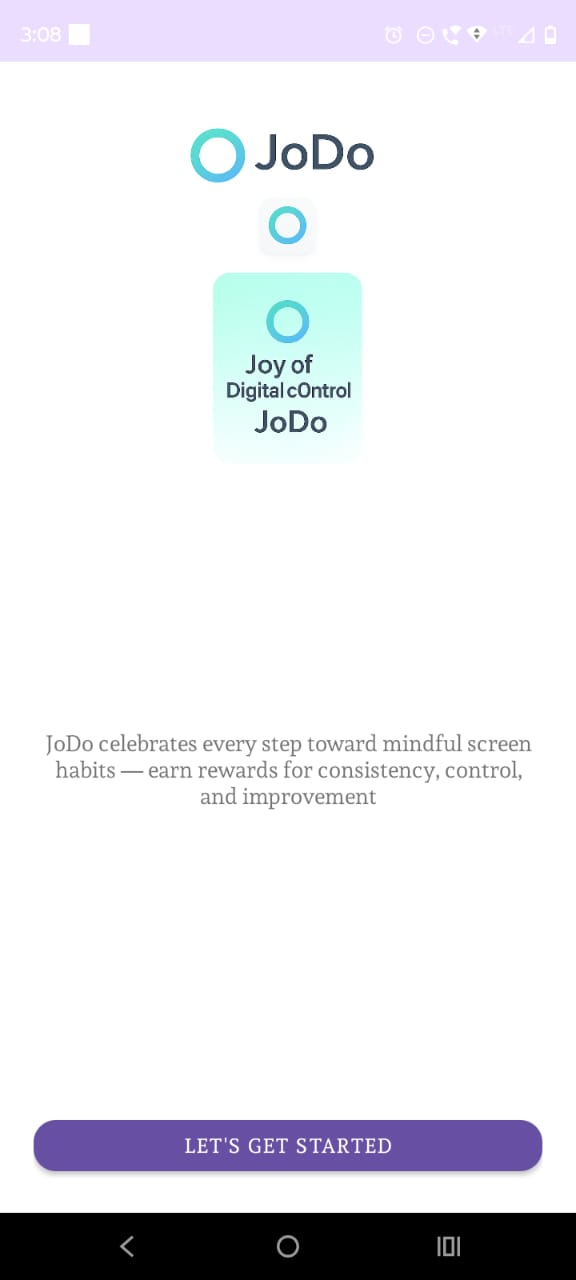
\includegraphics[width=0.50\linewidth,height=0.50\textheight, keepaspectratio]{get-started-screen.jpeg}
        \hspace{0,3cm}
        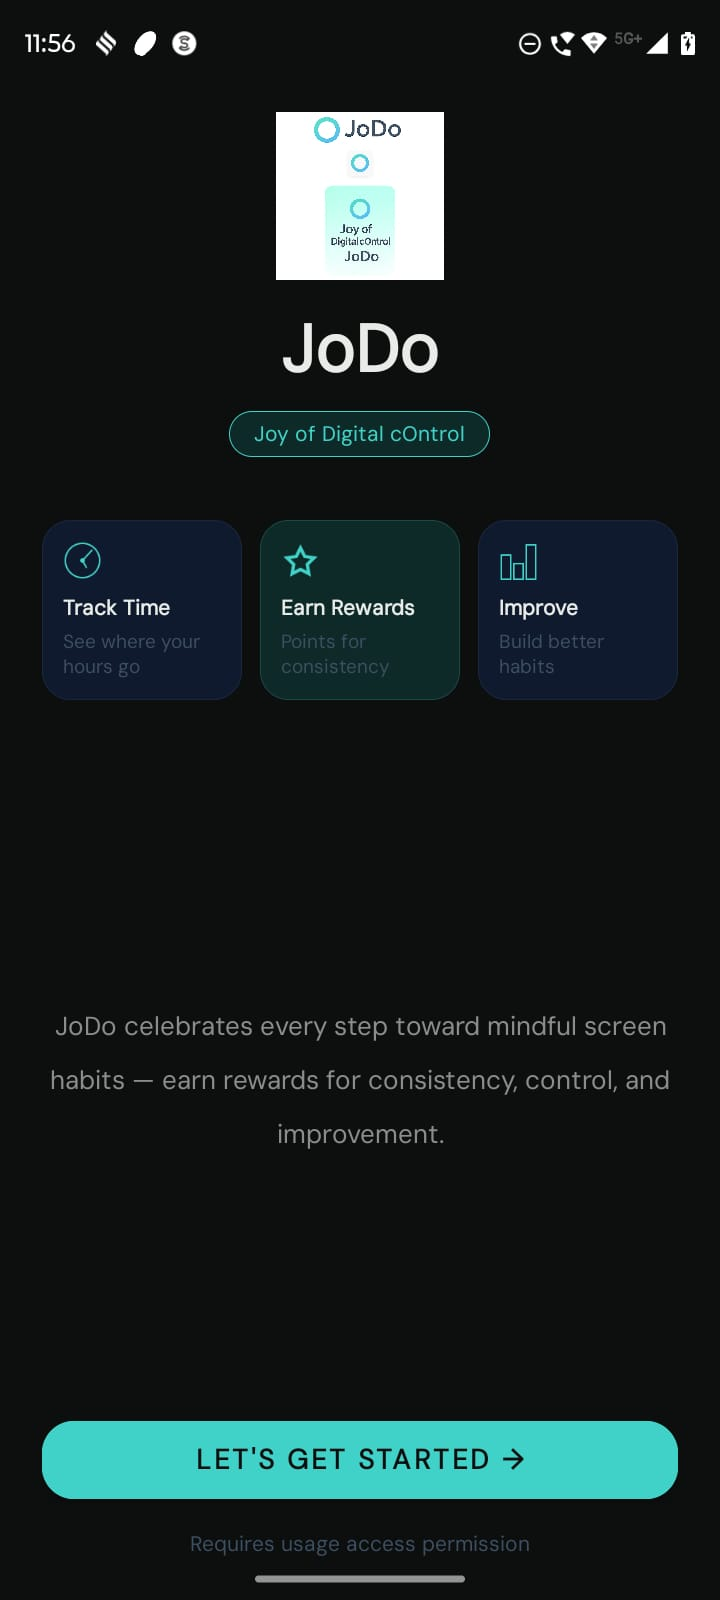
\includegraphics[width=0.50\linewidth, height=0.50\textheight, keepaspectratio]{new_get_started_screen.jpeg}
    
         \vspace{0.5cm}
    
        % 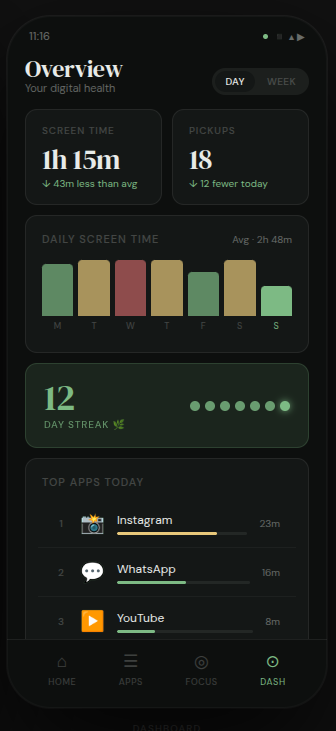
\includegraphics[width=0.45\linewidth]{JoDo new UI design/dashboard.png}
        % 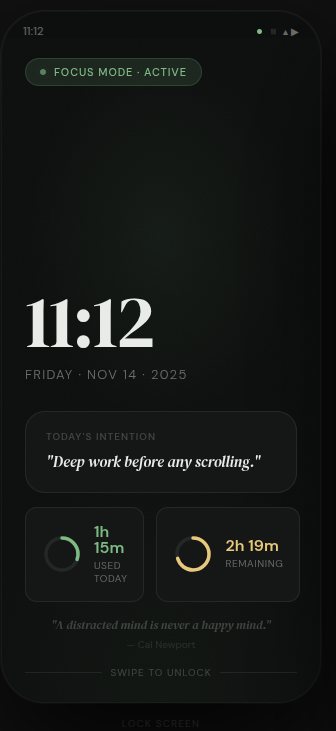
\includegraphics[width=0.45\linewidth]{JoDo new UI design/lock_screen.png}
    
        \caption{Get Started screen old (left)vs new UI (right)}
        \label{fig:ui_get_started screen}
    \end{figure}
\end{enumerate}
\subsection{To Do}
\begin{enumerate}
    \item Store upload status at server side.

    \item Only consider those users for weekly competition which are joined atleast 7 days before.
    \item Plan for ethics committee approval for user study.
    \item Republish app with latest code and updated privacy policy.
\end{enumerate}
\section{April 07 2026  - April 15 2026}
{\bf No. of Hours: 10}
\subsection{Migration from 4KB page size to 16KB page size}
\begin{enumerate}
    \item Historically, Android has supported 4KB page sizes, which has optimized system memory performance for the average amount of total memory that Android device have typically had.
    \item Begining with Android 15, AOSP supports devices that are configured to use a page size of 16KB.
    \item As device manufucturers continue to build devices with larger amount of physical memory(RAM), many of these devices will adopt 16KB (and eventually higher) page size to optimize device's performance.
    \item \textbf{Benefits and Performance Gain: } 
    Devices configured with 16KB page use slighly more memory on average, but also gain various performance improvement for both system and apps:
    \begin{enumerate}
        \item Lower App launche times while the system is under memory pressure. 3.16 \% lower on average.  with more significant improvement on some apps (upto 30 \%) improvement,
        \item Reduced power draw on App launch. 4.56 \% redunction on average.
        \item Fast camera launch: 4.48 \% fast camera launch (Irrelavent to our app)
        \item  Improved system Boot time: improved by 8 \% on an average (Irrelavent to our app).
    \end{enumerate}
\end{enumerate}
\subsection{APK Analysis Report from Android Studio}
\begin{enumerate}
    \item   \begin{figure}[H]
        \centering
        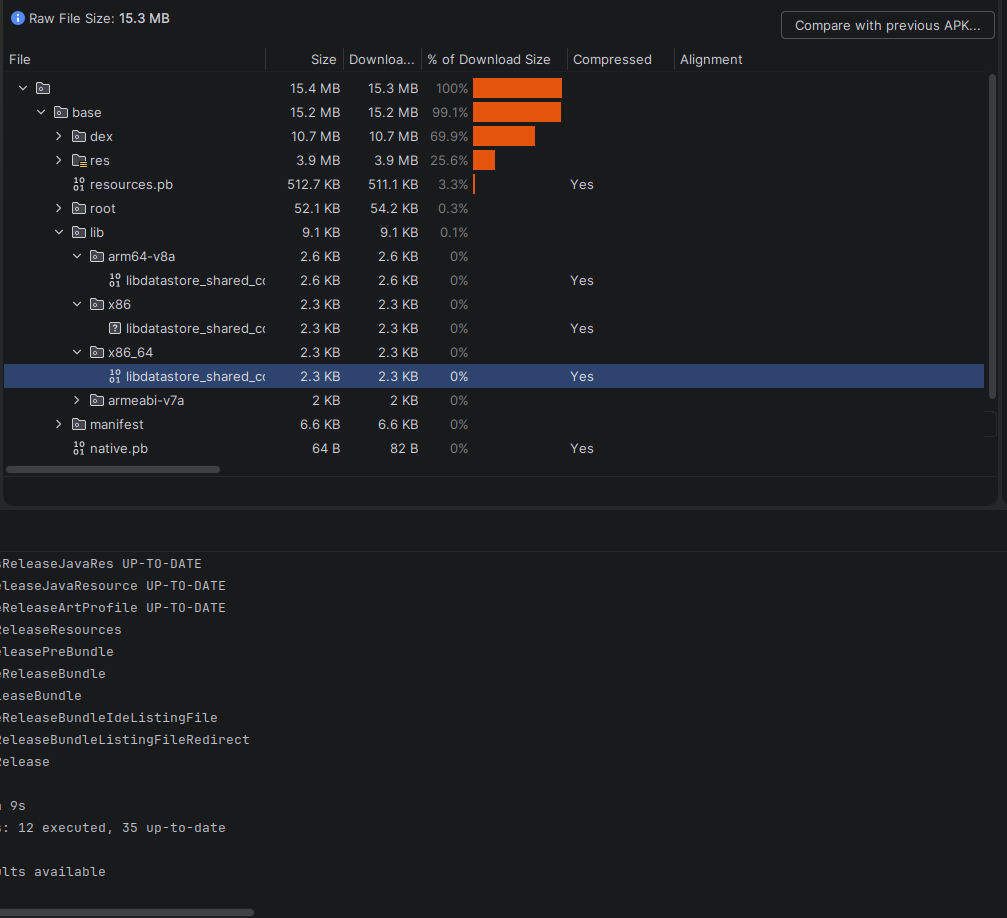
\includegraphics[width=0.50\linewidth,height=0.50\textheight, keepaspectratio]{apk_analysis.png}
    
        \caption{APK analysis report from android studio}
        \label{fig:apk_analysis_report_from_android_studio}
    \end{figure}
\end{enumerate}
\subsection{Code or Config Changes}
\begin{enumerate}
    \item Our App does not require any code change as our apk does not have any native pre-build library which depends on 16KB page size.
\end{enumerate}
\section{May 11 2026  - May 17 2026}
{\bf No. of Hours: 10}
\subsection{List of Task Completed:}
\begin{enumerate}
    \item Completed pilot study 2 with 3 users.
    \item Fixed bugs appeared in pilots study 2.
    \item Tested the new changes in all pilot devices.
    \item Increased version code and version number for new play store deployment.
    \item Created new .aab file for new deployment and verified that new .aab file is not corrupted.
\end{enumerate}
\section{May 18 2026 - May 19 2026}
{\bf No. of Hours 10}

\subsection{Proposed User study plan: }
\begin{enumerate}
    \item Create 2 week user study plan.
    \item Create on boarding form.
    \item Take approval from ethics committee.
    \item Create template for advertisement email.
    \item Create poster for user study.
    \item Start recruitment through mails and in person contact.
\end{enumerate}

\subsection{Summary of the paper: "In my defense, only three hours on Instagram": Designing
Toward Digital Self-Awareness and Well-being} \cite{karthik2026}
\begin{enumerate}
    \item Screen use pervades daily life, shaping work, leisure, and social connections while raising concerns for digital well-being.
    \item Theme of this paper is: \textbf{self-awareness, reflecting on one's digital behavior -as a critical pathway to digital well-being.}
    \item They created an app called: \textbf{WellScreen}
    \item Their main design for digital intervention is : They ask \textbf{Today's total usage time prediction} from the user in apps in particular category like social , entertainment, productivity and finance, shopping and food, and creativity. When the day ends they show the users their actual usages with color coded graphs and compare the estimated usage with the actual usage.
    \item At the end of the day they ask 5 question survey from the users (answer on the scale of 5-10) which includes: 
    \begin{enumerate}
        \item How satisfied are you with app usage?
        \item Did you meet your usage goal?
        \item How focused did you feel?
        \item How stressed did your usage make you feel?
        \item How in control did you feel?
        \item And a final self-reflection message from the user and their thoughts about their usage.
    \end{enumerate}
    \item They conducted user study with 25 participants mostly were university students over the period of 2 weeks.
    \item The goal of their user study was to find out: \textbf{How discrepancies between estimated and actual usage shaped digital awareness and well-being.}
    \item Participants  underestimate productivity and social and while overestimating entertainment app use. They showed a 10 \% improvement in positive effects ratting \textit{WellScreen} as \textbf{Moderately useful} (median SUS=80, IAM=14)..
    \item Their background literature includes: 
    \begin{enumerate}
        \item Digital Well-being as a concept: Digital well-being in \textit{HCI}, Digital well-being for college students.
        \item Self-awareness and Reflective Tools.
        \item Human-centered design of Digital well-being.
    \end{enumerate}
    \item \textbf{User Study Desgin and Method}:
    \begin{enumerate}
        \item \textit{The main goal of their was to examine how the recognizance of, and regular self-regulation on, college student's  estimated-actual gap in smartphone usage habits could advance our understanding of digital self-awareness and digital well-being.}
    \end{enumerate}
    \item \textbf{Participants and Recruitment} : They recruited participants through social media mainly through \textit{Reddit} community.
  \end{enumerate}

\subsection{Positive Points}
\begin{enumerate}
    \item Their study was focused mainly on behavior change,  they correlated screen time estimation and actual gap with individual differences which is good.
    \item They focused on individual digital self regulation and digital well-being, which could help in furthur developing individual specific digital well-being solutions which focuses on individual behaviour change rather than a group.
    \item Their work targeted what factor results in disparities.Why user generally ended up spending more than estimated? they tried to find out the digital well-being definitions with the help of statistics and user interview and actual screen usage pattern.
    \item They have done so many statistical analysis both on usage data as well as self-reported user data.
\end{enumerate}
\subsection{Negative Points}
\begin{enumerate}
    \item Their approached digital-well-being through self-awareness or self-reflection, showing the users the actual vs estimation, they haven't included any limiting strategy or motivational element.
    \item They haven't considered relapse in their study.
    \item Though their sample size is vary demographically but it was very small (only 25 people.)
\end{enumerate}
\section{May 20 2026  - May 24 2026}
{\bf No of Hours: 40}
\subsection{Pilot study 2 Report}
\begin{enumerate}
    \item The focus in pilot study 2 was mostly kept on ensuring the stability of the application across various devices before going for a larger user study for 2-3 weeks.
    \item Recruited 3 pilots with offline interaction from Hostel 14 (Master's CSE student).
    \item Before Downloading the app, all the 3 participants were asked to fill the \href{https://docs.google.com/forms/d/e/1FAIpQLScx9lyvxXDgia69XFIVvhky8M308N_4QHE2dzBAPSCAI8cA4Q/viewform}{consent form} .
    \item \textbf{Demographics: } Sex: male, age group: 22-26 for all the three participants.
    \item \textbf{Device Details: } Redmi 9I (Xiaomi), One-Plus, and Samsung.
    \item \textbf{Duration of the study:} 7 days.
    \item \textbf{Major Bugs/Crashes Found during Pilot study (Reported by Firebase Crash-analytics)}
    \begin{enumerate}
        \item \textbf{ AppDao\_Impl.insertUsageSummary:} java.lang.IllegalStateException - Room cannot verify the data integrity. Looks like you've changed schema but forgot to update the version number.
        \item \textbf{ AppDao\_Impl.insertApps:} java.lang.IllegalStateException - Room cannot verify the data integrity. Looks like you've changed schema but forgot to update the version number.
        \item \textbf{ AppDao\_Impl.insertUsageSummary:} java.lang.IllegalStateException - Room cannot verify the data integrity. Looks like you've changed schema but forgot to update the version number.
        
        \item \textbf{ActivityThread.generateForegroundServiceDidNotStartInTimeException: } Sometimes background service did not started from launcher.  
    \end{enumerate}
    \item \textbf{Applied Fixes:} 
    \begin{enumerate}
    \item Increased Room DataBase version Number in Android Client.
    \item Migrated foreground service launch from BootComplete receiver to HomeScreen, aligning with Android's background execution limitations.
    \end{enumerate}
\item \textbf{Feedback Recieved on Usability and UI: }
\begin{enumerate}
    \item One user wanted the lock screen should be option and permission for phone call should be asked when the user user enable JoDo as a lock-screen else do no ask during on-boarding.
    \item Give a setting button from which user can either set jodo as lock-screen or not.
    \item One pilot user wanted to use phone's default font instead of JoDo's font.
    \item One pilot user wanted to give option to set custom wallpaper on Home or lock Screen.
    \item All the three users rated 5/5  for to the  HomeScreen, app drawer, leaderboard, competition, and rewards design.
\end{enumerate}
\end{enumerate}


\subsection{Results from the Paper: "In my defense, only three hours on Instagram": Designing
Toward Digital Self-Awareness and Well-being \cite{karthik2026}}
\subsubsection{Estimated Vs. Actual Usage Gap}
\begin{enumerate}
    \item Their core finding is that people are very bad at estimating their own phone use - but in interesting, category-specific ways rather than uniformaly under or over-estimating.
    \item \textbf{What the Number shows?: }
    \begin{enumerate}
        \item \textbf{Social Media} was underestimated by \textbf{~9.6\%}. People used it more than they thought. Which is very natural by design of social media.
        \item \textbf{Productivity Apps} are under-estimated by \textbf{~16 \%}. People did more work than they themselve give credit for.
        \item \textbf{Entertainment} apps are over-estimate People thought that they were watching/gaming more than they actually were.
        \item At the \textbf{Aggregated level}, the estimated and actual totals didn't significantly differ -- meaning the error cancle each other out, which is why looking out at screen time only would have missed this all of this.
        \item \textbf{What predicts a smaller gap?} Self control was the most consistent factor across all the models (Table  4 \& 5 in paper) particularly for productivity apps and creativity apps, (this data doesn't reflect wether they are productive or creative or not, this results are based on the app usage data). This suggest that self - regulatory capacity is not just about \textbf{limiting} use, it's also linked to better \textit{awareness of one's behavior. } 
        \item \textbf{The Paradox (Table 6) :} smaller gaps (more accurate estimators) report higher satisfaction and stronger self-control day-to-day but also high stress and lower goal adherence. The authers suggest that accurate self-awareness may create a kind of performance pressure - once you know what you actually do, you feel more obligated to live upto your own predictions. Some participants even described skipping logging on days they expected irregularities, essentially avoiding the discomfort of seeing a large gap. 
    \end{enumerate}
\end{enumerate}

\subsubsection{WellBeing \& Affect Changes: }
\begin{enumerate}
    \item \textbf{The headline finding (Table 7) : } Participants showed a statistically significant \textbf{10 \% increase in positve affect}. (Cohen's d = 0.63, a large size effect size) after two weeks with WellScreen. Negative affect slightly decreased, but not significantly.
    \item \textbf{What's important to intercept here: }
    \begin{enumerate}
        \item Trait based measures - self-control and self-regulation - did \textit{not} change, which the authors correctly note is expected. These are stable personality-like traits unlikely to shift in two weeks. So the tool wasn't changing who \textit{people} are, but it was changing how they felt.
        \item The wellbeing improvement was likely driven by \textbf{shift in emotional interpretation} rather than actual behavior change. Participants describe a process of meaning-making  -- they reflected on their usage, justified it to themselves, and came away feeling more at peace with their habits. This mirrors psychological theories of self-discrepancy reduction (closing the gap between your "actual" and "ideal" self).
    \end{enumerate}
    \item \textbf{How participants' definition of digital well-being evolved: } This is one of the richer qualitative finding, At the start, most participants defined digital well-being narrowly as "time management" or "balance between real and virtual life". By the end their definitions had expanded to include 
    \begin{enumerate}
        \item \textbf{Intentionality: } - using technology purposefully rather than mindlessly.
        \item \textbf{Emotional Quality: } - whether digital interactions made them feel good or bad.
        \item \textbf{Digital footprint awareness: } - one participants even extended it to concern about data shared with corporation and AI systems.
    \end{enumerate}
    \item This conceptual broadening is significant: a two-week lightweight intervention shifted not just feelings, but how people think about what healty technology even means.
\end{enumerate}
\subsubsection{WellScreen Usability \& Self-Awareness}
\begin{enumerate}
    \item \textbf{Usability scores (Figure 2 from paper) : } The median \textbf{SUS scroe was 80}, which is considered "above average/acceptable". The median \textbf{IAM (invention appriateness) score was 14/20. } Indicating participants found it \textit{moderately} appropriate - useful, but not a perfect fit for everyone's context.
    \item  \textbf{The two-demisional breakdown (Figure 3)} is one of the most pratically interesting findings. Participants were mapped by self-control level and SUS score into four quadrants.
    \begin{enumerate}
        \item \textbf{High self-control + High usability:} Mostly willing to continue using it, but some felt the effort wasn't worth it ("it was me putting all the efforts")
        \item \textbf{High self-control + Low usability: } Mixed responses; wanted more than just data recording - wanted the tool to do something with their data.
        \item \textbf{Low self-control + Low Usability: } Evenly split; some found it eye-opening, others found it demotivating ("I just feel sad after looking at them")
        \item \textbf{Low self-control + High usability:} Strongest enthusiasm - this is the "sweet spot" where the  tool is most valuable, because the person genuinely need help and finds the tool easy to use. 
        \item \textbf{The key insight here} is that enthusiasm for a well-being tool require both a felt need (low self-control) and a good experience (high usability). If either is missing, the tool loses it's value.
    \end{enumerate}
    \item \textbf{Screen time as imperfect metric: } Participants also surfaced a fundamental measurement problem. Screen time conflates very different behaviors - some using YouTube as background music has to keep their screen on (inflating numbers), while a Spotify user doesn't. Falling asleep with TikTok open adds hours of "usage" that  wasn't conscious engagement. This reinforce the paper's broader argument that raw screen time is a poor proxy for digital well-being.
    \item \textbf{Value judgements in self-reflection: } Perhaps the most humanly interesting qualitative finding is that participants did'nt just \textit{report} their data. they \textit{judge} and \textit{defended} it. The title of the paper comes directly from a participants log entry justifying their screen time. People consistently distinguished "good use" (staying in touch with family, industry news) from "bad use" (mindless scrolling), and felt guilt even for activities they considered meaningful wjem the numbers looked high. WellScreen essentially functioned as a mirror that people felt compelled to justify themselves to.
\end{enumerate}
\subsubsection{Bottom line across all three RQs: }
\begin{enumerate}
    \item The paper's central argument holds up well in the data - self-awareness, not restriction, is the more promising path to digital well-being. The tool produced real emotional benefits without any explicit behavior-change mechanisms. simply by making the gap between perception and reality visible and prompting structured reflection.
\end{enumerate}
\subsection{Proposed User Study Design for JoDo}
\subsubsection{Overview}
A \textbf{two week deployment study} with college students, combining quantitative usage logging, validated survey at entry and exit, and semi-structured interviews - mirroring \textit{WellScreen's} three-phase structure but adapted to JoDo's reward-and-competition mechanics. 
\subsubsection{Phase 1: Entry Survey \& Interview (Day 0)}
\textbf{Survey Instruments} (same logic as WellScreen, capture stable traits as covariats)
\begin{enumerate}
    \item \textbf{BFI-10} for personality traits, since prior work link personality to technology use.
    \item \textbf{Brief self-control scale BSCS} - especially important for JoDo, because our competition design should theoritically benefit lower self-control users most.
    \item \textbf{Short-Self-Regulation-Questionair (SSRQ)}
    \item \textbf{PANAS-SF} for baseline positive and negative effects.
    \item Basic Demographics: age, gender, device type, self-reported daily screen time.
\end{enumerate}
\textbf{Entry Interview (30-45 minutes, via vedio call)}
\newline
Ask about: 
\begin{enumerate}
    \item Their current smartphone habits and pain points.
    \item Prior experience with any digital well-being tool(e.g. Forest, Appblock, StayFree, Minimalist launcher, etc.)
    \item Their understanding of what "digital well-being" means to them (This is important because WellScreen showed that the digital well-being definitions evolve, so it will give us some baseline to compare.)
    \item Initial reaction to \textit{JoDo} after a breif demo - do they find competition framing exiting or anxiety-inducing?
\end{enumerate}
\subsubsection{Phase 2: 2-Week Deployment}
\textbf{What to track Automatically (JoDo already does this) : }
\begin{enumerate}
    \item Daily screen time.
    \item Unlock count.
    \item App launch count.
    \item Points scored per day.
    \item Leader-board rank (daily/weekly)
    \item Wether the user interacted with \textit{Lock Now} voluntarily or not.
\end{enumerate}

\textbf{Daily/Weekly Micro-survey (Needs to be implemented with either Notification or Google form)}
\begin{enumerate}
    \item How satisfied were you with your phone use today? (1–7)
    \item Did you feel in control of your phone use today? (1–7)
    \item How stressed did you feel today? (1–7)
    \item Did the leaderboard/competition motivate you to use your phone less today? (1–7)
    \item Did you feel the rewards were fair/meaningful? (1–7)
    \item Did you voluntarily lock your phone today? (Yes/No)
    \item Since JoDo intervenes at the entry point (lock screen friction, app drawer transparency), We can ask participants to note on any given day whether they noticed the friction or found themselves reconsidering opening an app
\end{enumerate}
\subsubsection{Phase 3: Exit Survey \& Interview (Day 15)
}
\textbf{Exit Survey: }
\begin{enumerate}
    \item Repeat PANAS-SF, BSCS, SSRQ (to detect changes, note trait measures are unlikely to shift, but affect should)
    \item \textbf{System Usability Scale (SUS)} - same as \textit{WellScreen}
    \item \textbf{Intervention Appropriateness Measure (IAM)} - how fitting did JoDo feel in their life?
    \item Additional Items specific to JoDo:
    \begin{itemize}
        \item Did the competition feel motivating or stressful?
        \item Did the rewards feel meaningful or hollow or over time?
        \item Did you ever disable or ignore the lock screen friction? why?
    \end{itemize}
\end{enumerate}
\textbf{Exit Interview (30 - 45 mins)}
\begin{enumerate}
    \item How did their experience of competition evolved over the two weeks? (earlier enthusiasm vs late engagement)
    \item Did social comparison on leader-board feel supportive or discouraging?
    \item Did their definition of "digital well-being" change? (compare to entry time)
    \item What would make them using JoDo long term?
    \item Did they ever feel JoDo was unfair - e.g. getting penalized for actual productivity use?
\end{enumerate}
\subsection{Participants \& Recruitement}
Following WellScreen approach closely: 
\begin{enumerate}
    \item Target \textbf{N = 20 - 25} college students (aim for 20+ completion).
\item Recruit through IITB subreddits, department mailing list, whatsApp/telegram college group.
\item \textbf{Inclusion Criteria:} Android users, 18+ age, use their smartphone every day.
\item \textbf{Compensation:} Distribute daily and weekly rewards after exit interview, give drop-outs low price rewards if they won any.
\end{enumerate}
\subsection{Analysis Plan: }
\subsubsection{Quantitative: }
\begin{enumerate}
    \item Paired t-tests comparing entry vs. exit PANAS, BSCS, SSRQ scores. (with cohen's d effect size)
    \item Mixed effect regression: do daily points/ranks predicts daily satisfaction, self-control or stress? Do lower screen time days relates with higher positive affect?
    \item Track engagement decay: does daily survey completion or Lock Now usage drops after week 1 or firebase daily active user drops after week 1? This directly answers JoDo's key concern, Sustained motivation.
\end{enumerate}
\subsubsection{Qualitative: }
\begin{enumerate}
    \item Reflexive thematic analysis on interview transcripts. (same method as WellScreen)
    \item Code for: motivation dynamics, competitive pressure, perceived fairness of rewards, habitual vs intentional use.
\end{enumerate}
\subsection{Study Timeline Summary
}
\begin{table}[h]
\centering
\caption{Data Collection Instruments and Timeline}
\label{tab:data-collection}
\renewcommand{\arraystretch}{1.4}
\begin{tabular}{>{\raggedright\arraybackslash}p{4.5cm} 
                >{\raggedright\arraybackslash}p{5.5cm} 
                >{\raggedright\arraybackslash}p{3cm}}
\toprule
\textbf{Data Type} & \textbf{Instrument} & \textbf{Timing} \\
\midrule
\rowcolor{lightgray}
Demographic information 
    & Custom survey 
    & Day 0 \\
Personality \& self-control traits 
    & BSCS, SSRQ, BFI-10 
    & Day 0 and Day 15 \\
\rowcolor{lightgray}
Emotional wellbeing 
    & PANAS-SF 
    & Day 0 and Day 15 \\
Daily wellbeing \& rank perception 
    & Custom daily survey 
    & Days 1--14 \\
\rowcolor{lightgray}
Automatic usage logs 
    & JoDo app (screen time, unlocks, launches) 
    & Days 1--14 \\
Usability \& appropriateness 
    & SUS, IAM 
    & Day 15 \\
\rowcolor{lightgray}
Qualitative experience 
    & Semi-structured interviews 
    & Day 0 and Day 15 \\
\bottomrule
\end{tabular}
\end{table}
All validated instruments (BSCS,SSRQ,PANAS-SF,SUS,IAM) are publicly available and have been widely used in HCI and psychology with no unknown risks to participants.
\section{Risks and Benefits}
\textbf{Participants' Risks:}
This study poses \textbf{minimal risks} to participants.The primary potential risk is mild psychological discomfort arising from increase awareness of one's own smartphone usage,particularly if participants feel their usage is higher than they expected or if they rank low on leader-board.This is inherent and minor risk of any self-monitoring study.To mitigate this:
\begin{enumerate}
    \item Participants are informed before enrollment that leader-board ranking are relative and do not reflect personal worth or academic ability
    \item Participants are reminded at on-boarding and in the daily survey that they may withdraw at any point without penalty.
    \item The daily survey include an open-ended reflection field where any distress can be noted and followed up by research team
    \item No data will be shared with any third party including participant's institutions
\end{enumerate}
There are no psychological risks associated with participation.JoDo does not collect any personally identifiable information beyond what is voluntarily provided by participants.
\textbf{Potential Benefits:}
\begin{itemize}
    \item Participants may develop greater self-awareness of their smartphone habits
    \item Participants may experience improve positive affect,consistent with prior work on reflective digital well-being interventions
    \item Participants will contribute to research that could inform the design of more effective and autonomy preserving digital well-being tools
    \item Participants will receive financial compensation upto 1000 (INR).
\end{itemize}
\section{Informed Consent}
Informed consent will be obtained from all the participants prior to any data collection.. The consent process will include:
\begin{itemize}
    \item A written Participant Information Sheet explaining the study purpose,procedures,risks,benefits,and rights
    \item A signed consent form confirming voluntary participation,right to withdraw,and agreement to audio recording of interviews
    \item Verbal confirmation of consent at the start of each interview
\end{itemize}
Participants under 18 age will not be enrolled.Consent form will be stored securely and separately from research data.
\section{Data Privacy and Storage}
\begin{enumerate}
    \item All data will be anonymized using participant ID codes before analysis
    \item Interview recordings will be transcribed and then deleted within 30 days of transcription
    \item Anonymized transcripts and survey data will be stored on password-protected IIT Bombay servers
    \item No personally identifiable information will appear in any publication or report
    \item Data will be retained for a maximum of 5 years following study completion, after which it will be securely deleted
    \item The study complies with IIT Bombay data privacy policies and applicable Indian data protection guidelines
\end{enumerate}
\section{Compensation and Reward Structure}

Unlike conventional study compensation, JoDo's reward system is integral 
to the intervention itself --- the rewards are not external payments for 
participation but are the motivational mechanism being studied. 
Participants are not being paid to complete surveys or interviews; rather, 
they are competing within the app as part of the natural study experience.

The reward structure across the two-week deployment period is as follows:

\subsection*{Daily Rewards}
The top-performing participant on the daily leaderboard receives a cash 
voucher worth \rupee100, distributed at the end of each 24-hour competition 
cycle (14 days $\times$ \rupee100 = \rupee1,400 total).

\subsection*{Weekly Rewards}
At the end of each of the two study weeks, the top 3 participants on the 
weekly leaderboard receive an IIT Bombay notebook and pen set (valued at 
approximately \rupee500 per set; 3 winners $\times$ 2 weeks = \rupee3,000 total).

\subsection*{End-of-Study Overall Rewards}
At the conclusion of the full two-week period, overall leaderboard 
standings determine the following prizes:
\begin{itemize}
    \item \textbf{1st Place} --- Sports Watch: \rupee3,000
    \item \textbf{2nd Place} --- IIT Bombay Hoodie: \rupee1,500
    \item \textbf{3rd--5th Place} --- Steel Bottle and Bag: \rupee1,000 each 
    (3 $\times$ \rupee1,000 = \rupee3,000)
\end{itemize}

\subsection*{Study Materials}
JoDo onboarding card printing cost: approximately \rupee500.

\subsection*{Estimated Total Budget}
\begin{table}[H]
\centering
\caption{Reward Budget Summary}
\renewcommand{\arraystretch}{1.4}
\begin{tabular}{>{\raggedright\arraybackslash}p{7cm}
                >{\raggedright\arraybackslash}p{3cm}
                >{\raggedright\arraybackslash}p{3cm}}
\toprule
\textbf{Item} & \textbf{Calculation} & \textbf{Amount (INR)} \\
\midrule
\rowcolor{lightgray}
Daily winner cash voucher & \rupee100 $\times$ 14 days & \rupee1,400 \\
Weekly IITB notebook + pen set & \rupee500 $\times$ 3 $\times$ 2 weeks & \rupee3,000 \\
\rowcolor{lightgray}
End-of-study: 1st place sports watch & 1 $\times$ \rupee3,000 & \rupee3,000 \\
End-of-study: 2nd place IITB hoodie & 1 $\times$ \rupee1,500 & \rupee1,500 \\
\rowcolor{lightgray}
End-of-study: 3rd--5th place (bottle + bag) & 3 $\times$ \rupee1,000 & \rupee3,000 \\
JoDo onboarding card printing & --- & \rupee500 \\
\midrule
\rowcolor{lightgray}
\textbf{Total Estimated Budget} & & \textbf{\rupee12,400} \\
\bottomrule
\end{tabular}
\end{table}

\subsection*{Ethical Considerations Regarding Performance-Based Rewards}

The committee's attention is drawn to three potential concerns with this 
structure, and our mitigation strategies for each:

\begin{enumerate}

\item \textbf{Undue inducement:} The reward amounts are meaningful but not 
so large as to compromise voluntary participation or cause participants to 
take undue risks. The maximum individual reward (a \rupee3,000 sports watch) 
is consistent with compensation norms for short-term research participation 
at Indian institutions. Non-monetary rewards (notebooks, hoodies, bottles) 
also serve as institutional mementos rather than pure financial incentives.

\item \textbf{Fairness and dropout risk:} Participants who fall behind on 
the leaderboard early may feel demotivated. To mitigate this, the daily 
leaderboard resets every 24 hours, giving every participant a fresh 
opportunity regardless of prior performance. The weekly leaderboard 
similarly resets after each week. Examining this fairness perception is 
explicitly one of the research questions of the study, and the daily 
survey includes items measuring how rank affects motivation and wellbeing.

\item \textbf{Non-winners feeling unrewarded:} All participants who 
complete the full two-week study, regardless of leaderboard outcome, will 
receive a certificate of participation from the Department of CSE, IIT 
Bombay, ensuring that completing the study has a tangible acknowledgement 
for all participants.

\end{enumerate}
\clearpage 
\bibliographystyle{apalike}
\end{document}